\section{LLD in Tool-Integrated GRPO Collapse}
This section examines the prevalence of LLD in tool-integrated GRPO and illustrates how sustained likelihood decay ($\epsilon \leq 0$) leads to catastrophic training collapse. All analyses in this section use the NQ dataset~\citep{kwiatkowski2019natural} unless otherwise stated.
\subsection{Likelihood Dynamic}
% To characterize the prevalence and evolution of LLD during training, we visualize the training trajectory in \cref{fig:dynamic}. The dynamics exhibit three distinct phases. 
% \textbf{Phase I (early stagnation).} The likelihood of correct responses remains nearly constant despite increasing rewards, indicating the onset of LLD. The subsequent phases correspond to the $\epsilon \leq 0$ regime, where likelihood strictly decreases. 
% \textbf{Phase II (steady decay, steps 60--120).} Likelihood declines slowly but consistently, while rewards continue to rise and gradient norms remain stable. \textbf{Phase III (acceleration, after step 120).} Likelihood drops sharply and coincides with a rapid increase in gradient magnitude (marked by the red star), leading to gradient explosion and eventual training collapse.
% We further provide a zoomed-in view showing that, although collapse is ultimately triggered by gradient explosion, instability and reward degradation emerge earlier.

To characterize the prevalence and evolution of LLD during training, we visualize the training trajectory in \cref{fig:dynamic}. The dynamics exhibit three distinct phases.
\textbf{Phase I (early stagnation).} The likelihood of correct responses remains nearly constant despite increasing rewards, indicating the onset of LLD. The subsequent phases correspond to the $\epsilon \leq 0$ regime, where likelihood strictly decreases.
\textbf{Phase II (steady decay).} Likelihood declines slowly but consistently, while rewards continue to rise and gradient norms remain stable (e.g., steps 60–120 in \cref{fig:dynamic}).
\textbf{Phase III (acceleration).} After a turning point (around step 120 in \cref{fig:dynamic}), likelihood drops sharply and coincides with a rapid increase in gradient magnitude (marked by the red star), leading to gradient explosion and eventual training collapse.
We further provide a zoomed-in view showing that, although collapse is ultimately triggered by gradient explosion, instability and reward degradation emerge earlier.
% \begin{figure}[h]
%     \centering
%     \vspace{-2pt}
%     \includegraphics[width=0.9\linewidth]{images/llds.pdf}
%     \vspace{-6pt}
%     \caption{
%         Evolution of token 
%     }
%     \vspace{-4mm}
%     % \label{fig:feedback_likelihood}
% \end{figure}
\subsection{LLD Death Spiral}
% Let $\hat{\y} = (\y_{0}, \y_{1}, \ldots, \y_{T})$ denote the feedback-masked trajectory; a tuple $(\x, \hat{\y}^+)$ and a 
In \cref{fig:dynamic}, we observe an accelerated decline in response likelihood as training progresses. We formalize the resulting accelerated likelihood decay as an LLD death spiral.
\begin{definition}[Informal LLD Death Spiral]
Consider a policy update from $\pi_{\theta_s}$ to $\pi_{\theta_{s+1}}$.
We say the system enters an \emph{LLD Death Spiral} if the policy evolution follows the self-reinforcing pattern
\[
\mathrm{LLD}_s
\;\Longrightarrow\;
C_s^{\mathrm{low}}
\;\Longrightarrow\;
\mathrm{LLD}_{s+1},
\qquad
\varepsilon_{s+1} < \varepsilon_s \le 0,
\]
where $\mathrm{LLD}_s$ denotes lazy likelihood displacement at iteration $s$, and $C_s^{\mathrm{low}}$ denotes low-confidence trajectories whose likelihood decreases under $\pi_{\theta_s}$.
% The transition $\mathrm{LLD}_t \!\Rightarrow\! C_t^{\mathrm{low}}$ reflects that likelihood decay leads to increasingly diffuse predictions, while % $C_t^{\mathrm{low}} \!\Rightarrow\! \mathrm{LLD}_{t+1}$ occurs because low-confidence \emph{incorrect} responses often share actions with correct ones, inducing stronger negative-gradient interference (cf.~\cref{eq:GWHES-tool}).% Repeated iterations therefore accelerate likelihood decay, forming a self-perpetuating collapse.
\vspace{-2mm}
\end{definition}
A formal definition is provided in~\cref{sec:f_lld_s}, and the mechanism is visualized in~\cref{fig:effect_of_ld}. Beyond the acceleration phase shown in~\cref{fig:dynamic}, we further present additional empirical evidence of the LLD death spiral in the following section.
% \begin{definition}[LLD Death Spiral]
% Consider a tuple $(\x, \hat{\y}^+)$ and a policy update from 
% $\pi_{\theta_{t}}$ to $\pi_{\theta_{t+1}}$.  
% We say the system enters an \emph{LLD Death Spiral} if the policy evolution exhibits the following
% self-reinforcing progression:
% \[
% \mathrm{LLD}_{t}
% \;\Longrightarrow\;
% C^{\mathrm{low}}_{t}
% \;\Longrightarrow\;
% \mathrm{LLD}_{t+1}, \quad  \epsilon_{t+1} < \epsilon_t \leq 0
% \]
% where $\mathrm{LLD}_t$ denotes lazy likelihood displacement at time $t$ with decreasing likelihood ($\epsilon_t \le 0$), and $C^{\mathrm{low}}_t$ denotes low-confidence trajectories whose likelihood decreases under $\pi_{\theta_t}$.
% The transition $\mathrm{LLD}_t \Longrightarrow\ C^{\mathrm{low}}_t$ reflects that degraded likelihood leads to increasingly diffuse predictions, while the transition $C^{\mathrm{low}}_t \Longrightarrow\ \mathrm{LLD}_{t+1}$ occurs because low-confidence \emph{incorrect} responses often contain actions similar to those in correct responses, inducing a larger value in~\cref{eq:GWHES-tool} and thus a stronger negative-gradient influence.
% When these effects compound across iterations, the likelihood decay accelerates, creating a self-perpetuating collapse that we refer to as the \textbf{LLD Death Spiral}.
% \xl{Big Issue!!!! Reviewers will want to understand why this is a spiral rather than just a monotonic decay? When you mentioned this can you provide justification. At least you have empirical evidence in Figure 2: ``The acceleration phase (after step 120) exhibits superlinear decay: the likelihood drops by 0.5 in steps 120 versus 0.2 in steps 60, demonstrating that the rate of decline increases—the hallmark of a self-reinforcing spiral rather than monotonic decay.''
% }
% represents low-confidence trajectories whose overall likelihood continues to decline, yielding increasingly diffuse output distributions. The lower-confidence \emph{incorrect} responses often share prefix structures with the correct ones, creating higher prediction-error similarity and thereby \emph{intensifying} likelihood displacement. As this reinforcement compounds, the likelihood decay accelerates, forming the \textbf{LLD Death Spiral}.
\subsection{Empirical Evidence for LLD Death Spiral}
We demonstrate the LLD Death Spiral through \textit{accelerated entropy explosion} and \textit{accelerated per-sample LLD}. 
\\
\noindent\textbf{Accelerated Per-Sample LLD.}
We conduct a controlled study on the NQ dataset~\citep{kwiatkowski2019natural} to examine how GRPO training affect the likelihood of correct responses. Using Qwen2.5-3B-Ins~\citep{yang2024qwen2}, we generate eight rollouts per question and retain only samples containing both correct and incorrect responses. For each question, we reinitialize model parameters, apply a single GRPO update, and measure the average log-likelihood change of correct responses:
\begin{equation}\label{eq:LL change}
\Delta(\x)
:= \frac{1}{N^+} \sum_{i=1}^{N^+} \sum_{t=0}^{T_i}
\left[
\ln \pi_{\theta'}(\y_{i,t}^+ \mid \x)
-
\ln \pi_{\theta}(\y_{i,t}^+ \mid \x)
\right],
\end{equation}
where $N^+$ denotes the number of correct responses. As shown in \cref{fig:effect_ld_a}, likelihood degradation emerges as training progresses (\textcolor{orange}{orange} curve). During the acceleration phase (iterations 120--140), this effect intensifies into an \emph{LLD death spiral}, with $>$ 50\% samples exhibiting likelihood drops.
\begin{figure}[h]
\centering
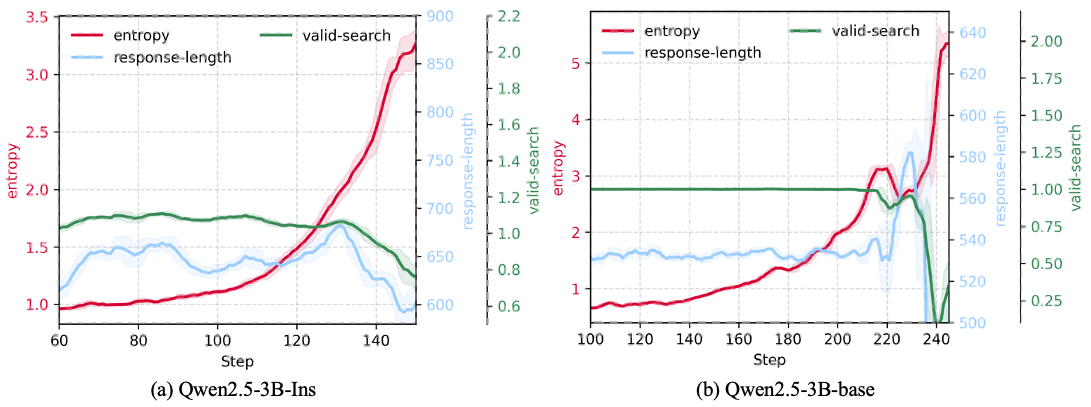
\includegraphics[width=\linewidth]{images/entropy_fig.png}
% \vspace{-2mm}
\caption{We visualize the evolution of entropy, response length, and valid-search ratio during training. For both Qwen2.5-3B-Instruct and Qwen2.5-3B-Base, entropy rises sharply prior to collapse, indicating severe likelihood displacement.}
\label{fig:entro_dyn}
\vspace{-3mm}
\end{figure}
\\
\noindent\textbf{Accelerated Entropy Explosion.}
\Cref{fig:entro_dyn} shows the evolution of entropy, response length, and valid-search ratio for Qwen2.5-3B-Ins and Qwen2.5-3B-Base. For both models, token entropy increases slowly in early training, consistent with the slow-LLD regime in \cref{fig:dynamic}, and then accelerates sharply during the LLD acceleration phase. This entropy surge reflects the LLD death spiral: accumulating low-confidence responses induce increasingly diffuse token distributions, further amplifying likelihood decay and instability. Notably, response length and valid-search frequency remain nearly constant, indicating that the entropy growth and likelihood degradation are driven by LLD rather than longer trajectories or increased tool usage.
\subsection{Why Tool-Integrated (TI) GRPO Amplifies LLD}\label{sec:correct-actions}
\begin{figure}[t]
    \centering
    % \vspace{-2pt}
    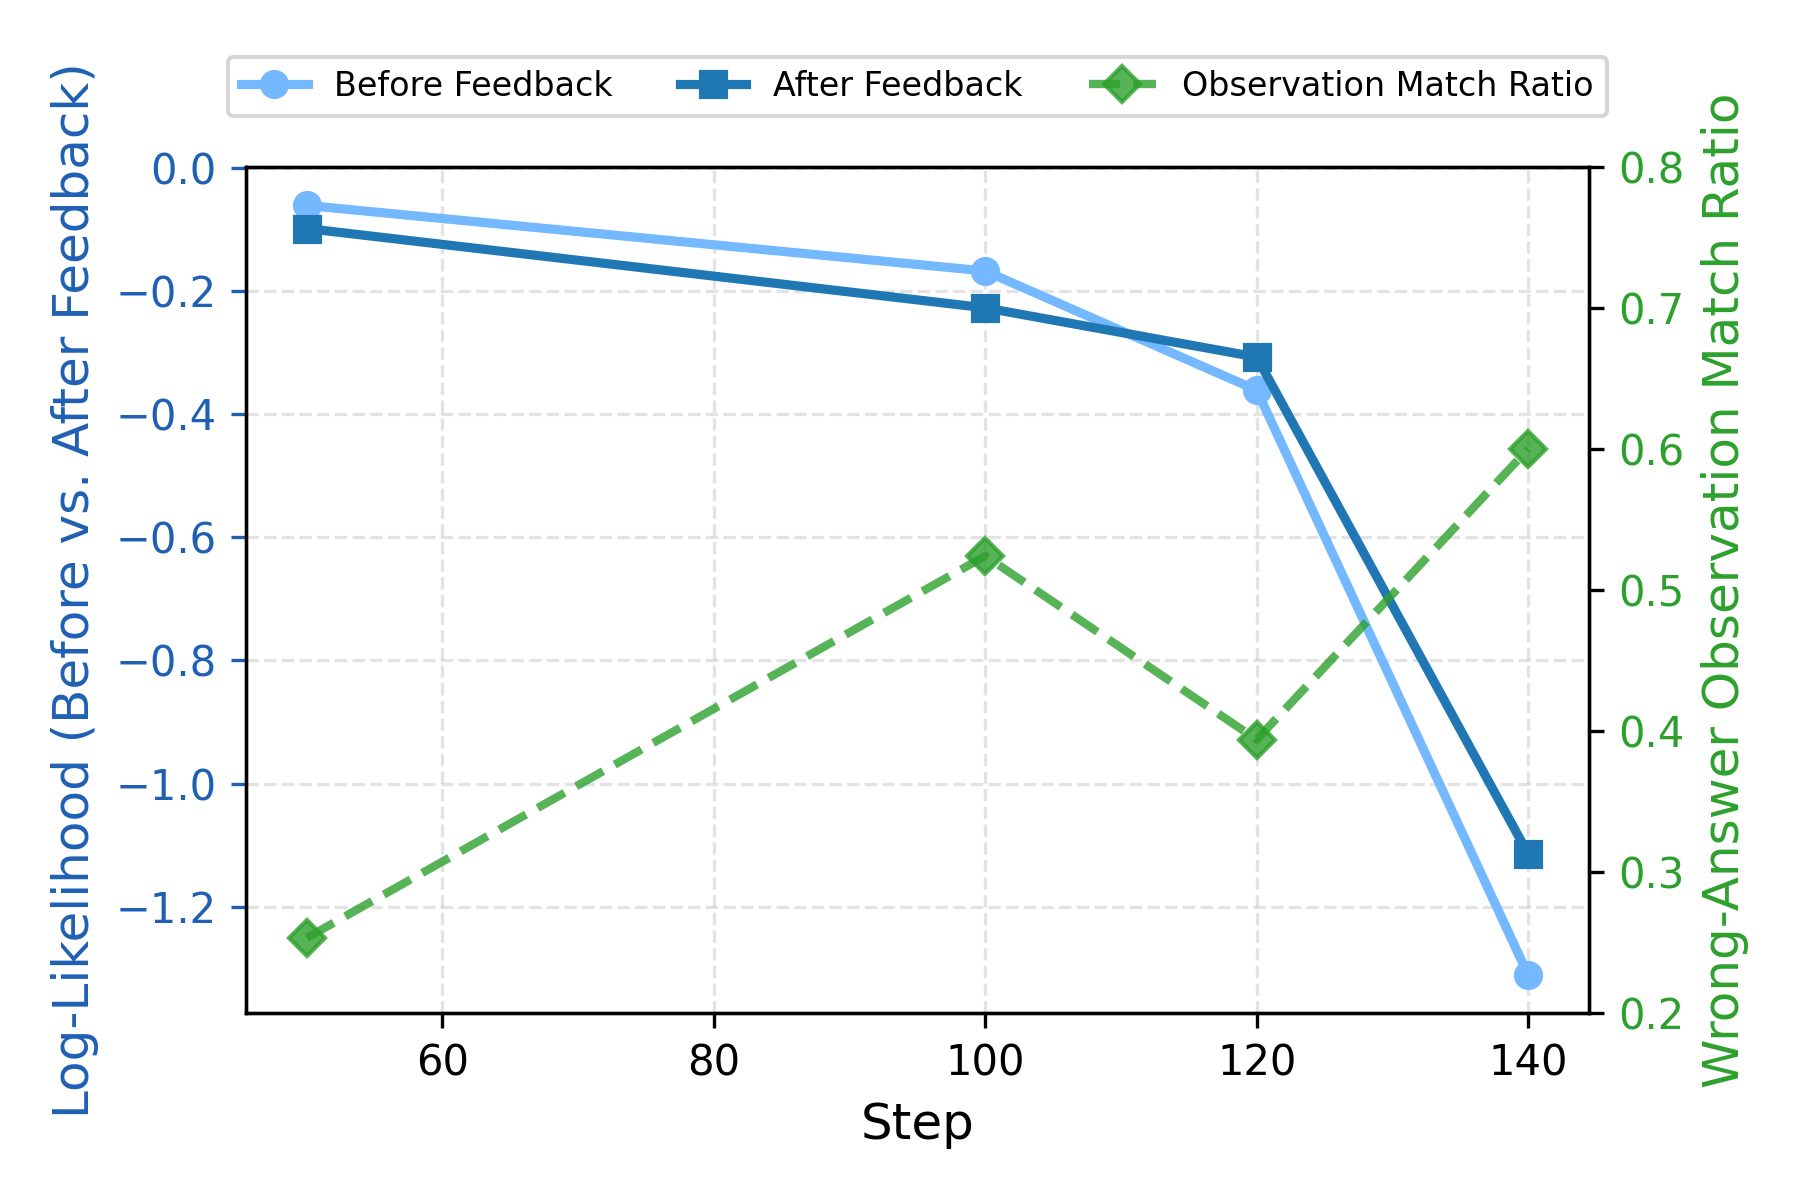
\includegraphics[width=\linewidth]{images/cross_logprob_fixed.png}
    \vspace{-3pt}
    \caption{
        Evolution of token log-likelihood (measured before vs. after feedback; left axis) and the observation-match ratio for wrong answers (right axis). With training, both likelihoods drop while the overlap between tool observations in incorrect and correct trajectories increases, suggesting many incorrect responses begin with a correct search, which skews likelihood estimates and contributes to LLD.
    }
    \vspace{-5mm}
    \label{fig:feedback_likelihood}
\end{figure}
We then show that the severity of LLD in TI-GRPO stems from two interacting factors predicted by \cref{the:infom} and demonstrated in \cref{fig:effect_ld_b}: high response similarity between correct and incorrect trajectories, and low likelihood responses that induce large prediction-error weights.
\\
\textbf{Frequent correct actions in incorrect responses.} Our analysis on Qwen2.5-3B-Ins that trained on the NQ dataset reveals a striking pattern: correct actions frequently appear within otherwise incorrect responses. Specifically, in TI GRPO, the first response action typically formulates a search query, whose correctness increases steadily during training regardless of final answer. We label the first action of incorrect responses as correct if its retrieved documents match those of a correct response. As shown in Fig.~\ref{fig:feedback_likelihood}, this accuracy (\textcolor{green}{green} line) is initially low but rises sharply, reaching $\sim$60\% by step 140, indicating high similarity on the first action between correct and incorrect trajectories. At the same time, the likelihood of the first action (\textcolor{cyan}{light blue}) decays faster than that of the second action (\textcolor{blue}{blue}): although initially higher due to the second action conditioning on OOD feedback, it drops below the second action around step 110, where first-action correctness reaches $\sim$50\%. After step 120, this decay accelerates sharply, where low-likelihood incorrect prefixes further amplify degradation. As LLD intensifies, the likelihood of the first action collapses, and the model begins producing random, nonsensical tokens (Appendix, Fig.~\ref{fig:geeh-incorrect}), rendering responses effectively unusable even before full training collapse. These results motivate mitigating unintended penalization of correct actions within incorrect trajectories (see \cref{sec:discuss}).
\begin{figure}[t]
% \vspace{-2mm}
    \centering
    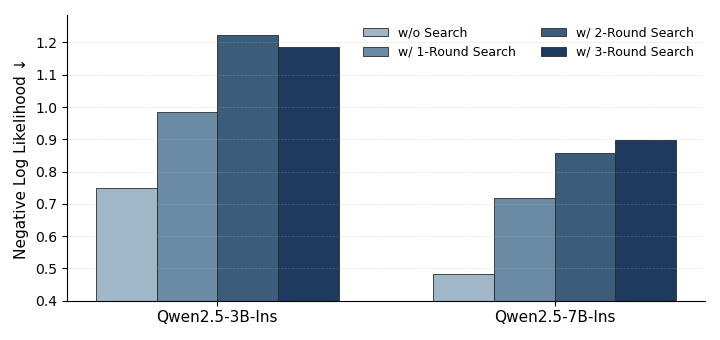
\includegraphics[width=\linewidth]{./images/off_policy.png}
    % \vspace{-2mm}
    \caption{Effect of off-policy tool context on negative log-likelihood. Increasing the number of tool-interaction rounds consistently reduces response likelihood.}
    \label{fig:off_policy_nll}
    \vspace{-6mm}
\end{figure}
\\
\noindent\textbf{Low Likelihood reasoning after tool feedback.}
A second factor that amplifies LLD is the use of OOD tool feedback as a conditioning context. They introduce a persistent distribution mismatch between the policy and its input context, systematically reducing the likelihood assigned to subsequent actions and increasing negative log-likelihood. As shown in \cref{fig:off_policy_nll}, computed on the first 50 NQ training samples, this effect strengthens with the number of tool-interaction rounds, producing a monotonic increase in NLL for both Qwen2.5-3B-Instruct and Qwen2.5-7B-Instruct models. 